\documentclass{article}

\usepackage[final,nonatbib]{neurips_2023}

\usepackage[utf8]{inputenc}
\usepackage[T1]{fontenc}
\usepackage{hyperref}
\usepackage{url}
\usepackage{booktabs}
\usepackage{amsfonts}
\usepackage{nicefrac}
\usepackage{microtype}
\usepackage{xcolor}

\usepackage{graphicx}
\usepackage{caption}
\usepackage{subcaption}

\usepackage{listings}
\lstset{
    basicstyle=\ttfamily,
    breaklines=true,
    breakatwhitespace=true,
}


\title{LOLCATS: Leveraging Obscure Lexical Conventions And Tenuous Synonyms in computer science research}


\author{%
  Kyle Roth \\
  DIRO \\
  Université de Montréal \\
  Montréal, QC, Canada \\
  \texttt{kyle.roth@umontreal.ca} \\
  \And
  Georges Bélanger\thanks{An especially cool guy.} \\
  Affiliation \\
  Address \\
  \texttt{email} \\
  \And
  Alex Fulleringer\thanks{An especially cool guy.} \\
  Concordia University \\
  Montréal, QC, Canada \\
  \texttt{alexfulleringer@gmail.com} \\
}


\begin{document}


\maketitle


\begin{abstract}
  We did some stuff!
\end{abstract}


\section{Introduction}
Recent developments in natural language processing have shown that in-context learning allows large language models (LLMs) to quickly adapt to new tasks by using natural language instructions and a few demostrations as a prompt.
Specifically, this investigations examines how using the ART framework~\cite{paranjape2023art}, we can create and teach the LLM to use tools for Long Document Summarization.

In the ART paper, they generate automatic multi-step decompositions for new tasks by selecting decompositions of related tasks in the task library, and then select and use tools in the tool library alongside LLM generation.
We simplify the framework and only focus on constructing few-shot prompts for long document summarization that learn information onto external tools. We leverage ART's program grammar, but create new tools specically designed for summarization of large documents splitted into chunks of text.


\section{Background}
Apart from the ART paper, another work that uses tools with an LLM is Toolformer \add{cite}.
However, different from ART, Toolformer was finetuned to learn how to use tools, as opposed to in-context learning. The advantage of our approach is that you can switch LLM without the need of finetuning.

Other relevant recent work proposes prompting LLMs to mimic a chain of thought (CoT) for multi-step reasoning by stating in the prompt to think Step-by-step \add{cite}.

Finally, state-of-the-art approaches for long document summarization include the following:
Top Down Transformer (Long Document Summarization with Top-down and Bottom-up Inference)
LongT5: Efficient Text-to-Text Transformer for Long Sequences
Pegasus X: Investigating Efficiently Extending Transformers for Long Document Summarization and Document Summarization with Text Segmentation \add{\cite}.


\section{Methodology}
%- provide tools that are analogous to long term memory in humans

Our goal was to create a modified ART framework that allows for an LLM to read from, write to, and organize a form of long-term memory, without actually retraining model weights.
This would allow for the model to dynamically access previously stored information, as well as update its local repository with valuable data as it reads through prompts.
Given the finite context window of any LLM, ensuring that only relevant data is retrieved would be a crucial requirement of this system.
With these goals and constraints in mind, we chose a Python dictionary as the underlying data structure for persisting information.
A dictionary naturally organizes data into key-value pairs, which would naturally allow for organization and efficient retrieval based on the LLM selecting only relevant keys.
The LLM would load the information stored at keys it finds relevant to its current task, and organize the information it stores by choosing an appropriate key.

In the context of ART, this translates into the creation of three tools to accomplish our envisioned task. Firstly, we define \texttt{[list-keys]}, a tool that takes no inputs and returns a string containing all the keys in the dictionary.
Next we define \texttt{[write]}, this tool requires a key-value pair and writes the pair into the dictionary, updating the value stored under the key if it is already present.
Finally, we define \texttt{[read]}, a tool that takes a key as input and returns the information stored at that key in the dictionary.
Currently the tools save the dictionary to, and read it from, storage to ensure the long term stability of the data.

We demonstrate our tools by performing a summarization task on journal articles taken from DATASET HERE.
As is standard with ART prompts, demonstrations of the task are prepended to the prompt to provide the LLM an example of how to handle the task~\cite{paranjape2023art}.
Each article is split into multiple chunks that are fed one at a time into the modified ART framework, with the network choosing how to organize and persist data for later perusal.
At the end of each article, each entry in the dictionary is then fed back into the LLM and a complete summary is generated. Experiments, results, and their analysis are discussed below.

\section{Experiments}\label{section:experiments}

To effectively judge the usefulness of our method, we chose to evaluate on the abstractive summarization task. Unlike extractive summarization, in this task the summary is expected to be a concise representation that effectively communicates the key ideas in the text, rather than a composition of important phrases in the text. This is more like how humans generally summarize texts, and provides a stronger challenge for our method. We evaluated our method on the arXiv abstractive summarization dataset~\cite{cohan-etal-2018-discourse}. Texts in this dataset can be more than 300k tokens in length (see statistics in Figure~\ref{fig:length-hist}), which provides a good setting to test how well our method allows a model to use information from across long input.

\begin{figure}[!ht]
  \centering
  \begin{subfigure}{0.45\textwidth}
    \centering
    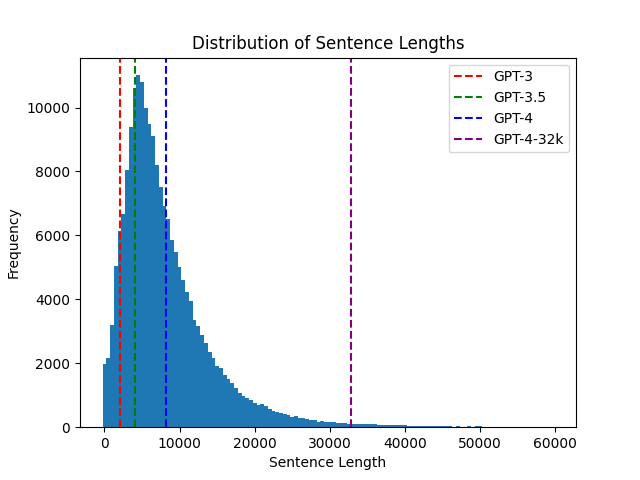
\includegraphics[width=\linewidth]{images/length_hist_train.png}
    \caption{Sentence lengths in the train set. The sentence lengths have mean 8,630.2, median 6,883.0, minimum 0, and maximum 329,071 (not visible).}\label{fig:train-hist}
  \end{subfigure}
  \hfill
  \begin{subfigure}{0.45\textwidth}
    \centering
    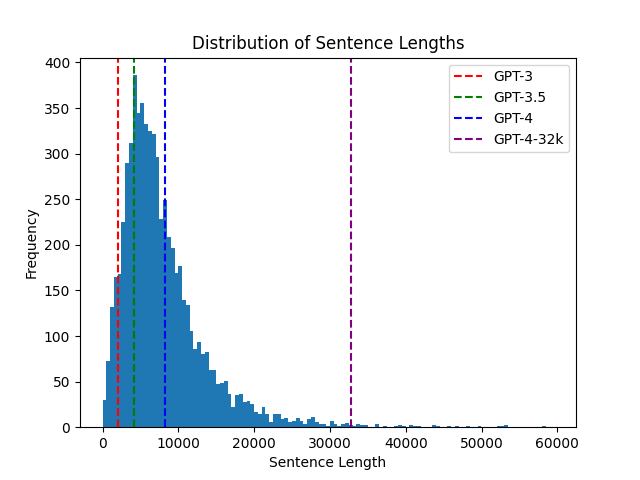
\includegraphics[width=\linewidth]{images/length_hist_validation.png}
    \caption{Sentence lengths in the validation set. The sentence lengths have mean 8,208.3, median 6,871.5, minimum 244, and maximum 109,442 (not visible).}\label{fig:val-hist}
  \end{subfigure}
  \caption{Distribution of sentence lengths (number of tokens) in the train and validation sets. For reference, the maximum context sizes for various GPT models are marked as vertical lines. Our method makes it feasible to summarize long documents without access to GPT-4 or GPT-4-32k.}\label{fig:length-hist}
\end{figure}

To this end, we designed three tools for the model to use: \texttt{[read]}, \texttt{[write]}, and \texttt{[list-keys]}; along with a prompt that explains the task and demonstrates how to use these tools to accomplish the goal of a good summary. The \texttt{[read]} and \texttt{[write]} tools each accept a short text key, and the text associated with the key is stored in a Python dict. This data is specific to each article, and is built by the model as it receives each chunk. The prompt specifically instructs the model to store information under meaningfully-named keys using \texttt{[write]}, and then to \texttt{[read]} all stored information during the last chunk in order to produce the final output.\footnote{See Appendix~\ref{section:prompts} for the text of the prompts used in this project.}

Each article is split into chunks of 15 sentences each. We would have preferred to make sure chunks did not cross section dividers, but this was not possible due to the preprocessing in the dataset.

\subsection{Prompt Variations}

We experimented with two variations on the original prompt, both of which ended up improving the performance. One we call ``compressed intermediates'', and the other we name ``rolling summary''.

For ``compressed intermediates'', we modify the examples to show the model storing text that looks more like compressed notes than a complete summary. This reduces the number of tokens in the prompt as well as in model generations, which decreases the chance that the final summarization will be too large for the model to summarize from. In this experiment we also increased the length of the keys used for \texttt{[read]} and \texttt{[write]}; e.g.~``regular-chaotic-motions'' became ``regular-chaotic-motions-smooth-curves''. This seems to reduce the frequency of key collisions when text discussing a single phenomenon is split across multiple chunks.

The prompt for ``rolling summary'' replaces the key names (``regular-chaotic-motions'', etc.) with ``current-summary'', and the stored summaries summarize both the current chunk and all previous chunks. The final example shows the model reading just the single key ``current-summary'' and combining it with the input chunk to produce the answer. Verbiage in the explanations is also slightly adapted to match these differences.


\section{Results}

We report metrics from the ROUGE family~\cite{lin-hovy-2003-automatic,ganesan2015rouge} for the three approaches on \texttt{n=10} samples from the validation set.

\begin{table}[!ht]
  \centering
  \begin{tabular}{c|c|c|c|c}
    \textbf{Method} & \textbf{ROUGE} & \textbf{ROUGE-2} & \textbf{ROUGE-L} & \textbf{ROUGE-L-Sum} \\
    \hline
    base            & 11.7           & 4.0              & 6.1              & 8.2                  \\
    compressed      & 29.4           & 9.7              & 15.1             & 23.1                 \\
    rolling         & 34.2           & 8.8              & 18.7             & 27.3                 \\
  \end{tabular}
  \vspace{0.5cm}
  \caption{Experimental results for each of the prompts described in Section~\ref{section:experiments} on 10 samples from the arXiv summarization dataset, evaluated on several ROUGE-based metrics.}\label{tab:results}
\end{table}

We observe clear improvement over the base prompt for the two modifications. While the sample size for this experiment was small,\footnote{The cost of this experiment with \texttt{n=10} was US\$16, so we would like more funds in order to validate that these changes improve performance.} we think the difference is significant because they make it possible for more stored information to be \texttt{[read]} when generating the final summary.



\section{Conclusion}

- context window is limiting to ART framework
- future work in fine tuning a model instead of using a frozen one.
- lightweight models may be more appropriate
- Could be used for better conversational AI

In this project we have designed and implemented tools to be used by an LLM to organize and store relevant data for long-term/future use.
We encountered difficulties in providing enough context for the LLM to properly use the tools, but found some success with simplified run strategies.
Future research avenues could involve using newer, bigger, LLMs that have larger context windows allowing for more varied tool use samples to be passed as part of the prompt.
Otherwise, it may be desirable to fine tune smaller models specifically to use tools and address long standing issues with LLM capabilities.
To achieve the goal of an AGI system, it will be necessary for it to diversify its problem-solving across many contexts.
Creating systems capable of learning to use tools may be an invaluable step along this path.

\bibliographystyle{neurips}
\bibliography{main}


\appendix

\section{Prompts}\label{section:prompts}

Here is the complete base prompt we used for our experiments. Unlike Paranjape et al.~\cite{paranjape2023art}, we do not experiment with dynamically varying the prompt in any way.


\begin{lstlisting}
  You are tasked with summarizing a long document that does not fit in the context window. We will show you chunks of the text to summarize one at a time, resetting your context window each time. Fortunately, you have access to three tools: [read], [write], and [list-keys], which you can use to read and write information to an external location that is accessible as you process later chunks. Here are a few examples of how you might use these tools when dealing with a chunk:

  ----BEGIN EXAMPLE----
  Input: (1/4) first , the curve is significantly smoother as a function of @xmath0 for larger @xmath44 . even more relevant is the fact that the single trajectory data ( @xmath45 ) may show current reversals that do not exist in the large @xmath44 data <SHORTENED FOR BREVITY> ( , ) for example .   notice also that in fig .   (  ) , at @xmath55 and @xmath56 , the deviations between the different ensembles is particularly pronounced .
  Q1: [write] (regular-chaotic-motions) The behavior of a system with regular and chaotic motions is a function of the number of trajectories and the location of the initial ensemble. The curves are smoother for larger numbers of trajectories, and single-trajectory data may show current reversals that do not exist in the large data set. The net drift of an ensemble can be closer to the behavior of an individual trajectory, and there is a dependence of the current on the location of the initial ensemble. The width of the ensemble also affects the details of the current and can cause illusory current reversals.
  #1:
  Q2: [EOQ]
  ----END EXAMPLE----

  In the example above, you write a short summary of the chunk to memory using [write]. This information will be accessible later, as you can see when we process the next chunk below:

  ----BEGIN EXAMPLE----
  Input: (2/4) these points are close to bifurcation points where some sort of symmetry breaking is clearly occuring , which underlines our emphasis on the relevance of specifying ensemble characteristics in the neighborhood of unstable behavior . <SHORTENED FOR BREVITY> however , there is only one instance of current - reversal , at @xmath65 .   note , however , that the current is not without structure  it changes fairly dramatically as a function of parameter .
  Q1: [read] regular-chaotic-motions
  #1: The behavior of a system with regular and chaotic motions is a function of the number of trajectories and the location of the initial ensemble. The curves are smoother for larger numbers of trajectories, and single-trajectory data may show current reversals that do not exist in the large data set. The net drift of an ensemble can be closer to the behavior of an individual trajectory, and there is a dependence of the current on the location of the initial ensemble. The width of the ensemble also affects the details of the current and can cause illusory current reversals.
  Q2: [write] (ensemble-effects) In the classical phase space for Hamiltonian or underdamped motion, dynamics depend on the initial conditions. However, when damping is introduced, the phase space consists of attractors, and the current is less likely to depend significantly on initial conditions. In the chaotic regime of a non-Hamiltonian system, the initial ensemble needs to be larger than a certain threshold for convergence, while in the regular regime, a single trajectory suffices as long as transients are discarded. We propose a modified definition of current that includes an empirically obtained cut-off to ensure convergence. We compare bifurcation diagrams with the current in a series of figures, noting that there is a single current reversal in the examined parameter range despite several bifurcations. The current changes dramatically as a function of the parameter, but only one instance of current reversal occurs.
  #2:
  Q3: [EOQ]
  ----END EXAMPLE----

  See how in the example above you read an existing summary, and used that information to help summarize the current chunk. You don't always have to read from storage; maybe you're summarizing the first chunk (1/n), or you don't need contextual info to summarize this chunk well. Now I’m going to show you how to use the `list-keys` tool:

  ----BEGIN EXAMPLE----
  Input: (3/4) the ensemble results on the other hand , even when converged , show statistical roughness .   ( b ) the ensemble results are consistent with barbi and salerno in general , although disagreeing in several details . <SHORTENED FOR BREVITY> note in particular in this figure that eyeball tests can be misleading .
  Q1: [list-keys]
  #1: regular-chaotic-motions, ensemble-effects
  Q2: [read] ensemble-effects
  #2: In the classical phase space for Hamiltonian <SHORTENED FOR BREVITY> current reversal occurs.
  Q3: [write] (bifurcations-and-reversals) The passage describes a study on the relationship between bifurcations and current reversals in a system. The authors used ensembles of particles to examine how their results converged as a function of various parameters. They found that not all bifurcations led to current reversals, but did not rule out the possibility that all current reversals are associated with bifurcations, which is Mateos' conjecture. The study differed from a previous one by Barbi and Salerno, who used single-trajectory results instead of ensembles of particles. The article concludes that the ensemble current provides significant information that cannot be obtained from a single-trajectory current.
  Q3: [EOQ]
  ----END EXAMPLE----

  In this final example, we show how you will output the final summary using [ans]:

  Input: (4/4) we see reversals without bifurcations in ( a ) whereas the zoomed version ( c ) shows that there are windows of periodic and chaotic regimes . <SHORTENED FOR BREVITY> each of the transitions from periodic behavior to chaos and back provides opportunities for the current to spike .
  Q1: [list-keys]
  #1: regular-chaotic-motions, ensemble-effects, bifurcations-and-reversals
  Q2: [read] regular-chaotic-motions
  #2: The behavior of a system <SHORTENED FOR BREVITY> current reversals.
  Q3: [read] ensemble-effects
  #3: In the classical phase space for Hamiltonian <SHORTENED FOR BREVITY> current reversal occurs.
  Q4: [read] bifurcations-and-reversals
  #4: The passage describes a study on the relationship between bifurcations <SHORTENED FOR BREVITY> from a single-trajectory current.
  Q5: [ans] This work delves into the relationship between bifurcations and current reversals in a driven, damped, and chaotic system, emphasizing the significance of considering ensembles of trajectories and their convergence properties when examining the current's behavior. It is discovered that not all bifurcations result in current reversals, and not all current reversals are linked to bifurcations. Nonetheless, a generalization of Mateos' conjecture is proposed, which suggests that bifurcations correspond to sudden current changes (spikes or jumps). This improved understanding aids in characterizing changes in the current's behavior as a function of parameter and is useful in identifying "hidden" bifurcations, providing a more comprehensive perspective on the system's dynamics.
  ----END EXAMPLE----
  Remember, you are summarizing a long document that does not fit in the context window, and we will only show you one chunk of the text now. {instructions} Here you go:

  Input: ({i}/{n}) {text}
  Q1:
\end{lstlisting}

Here, \texttt{\{text\}} is replaced with the text of the chunk, and \texttt{\{i\}} and \texttt{\{n\}} are replaced with the position of the current text in the chunks from the text. \texttt{\{instructions\}} is set with specific instructions for tool use for the first and last chunks; see the code repository for details.

\subsection{compressed intermediates prompt}

The change to the first example in the prompt is illustrative of the change effected in the intermediate notes produced with this version of the prompt:

\begin{lstlisting}
  * behavior is a function of the number of trajectories and the location of the initial ensemble * curves are smoother for larger numbers of trajectories * single-trajectory data may show current reversals not in the large data set * net drift of an ensemble can be closer to behavior of individual trajectory * current depends on location of the initial ensemble
\end{lstlisting}

Again, see the repository for details.


\end{document}
